%%%%%%%%%%%%%%%%%%%%%%%%%%%%%%%%%%%%%%%%%%%%%%%%%%%%%%%%%%%%%%%%%%%%%%%%%%%%%%%
%                       CARGA DE LA CLASE DE DOCUMENTO                        %
%                                                                             %
% Las opciones admisibles son:                                                %
%      12pt / 11pt            (tamaño del cuerpo de letra; no usar 10pt)      %
%                                                                             %
% catalan/spanish/english     (idioma principal del trabajo)                  %
%                                                                             % 
% french/italian/german...    (si necesitáis usar otro idioma adicional)      %
%                                                                             %
% listoffigures               (El documento incluye un Índice de figuras)     %
% listoftables                (El documento incluye un Índice de tablas)      %
% listofquadres               (El documento incluye un Índice de cuadros)     %
% listofalgorithms            (El documento incluye un Índice de algoritmos)  %
%                                                                             %
%%%%%%%%%%%%%%%%%%%%%%%%%%%%%%%%%%%%%%%%%%%%%%%%%%%%%%%%%%%%%%%%%%%%%%%%%%%%%%%

\documentclass[11pt,spanish,listoffigures,listoftables]{tfgetsinf}

%%%%%%%%%%%%%%%%%%%%%%%%%%%%%%%%%%%%%%%%%%%%%%%%%%%%%%%%%%%%%%%%%%%%%%%%%%%%%%%
%                     CODIFICACIÓN DEL ARCHIVO FUENTE                         %
%                                                                             %
%    Windows suele usar 'ansinew'                                             %
%    en Linux es posible que sea 'latin1' o 'latin9'                          %
%    Pero lo más recomendable es usar utf8 (unicode 8)                        %
%                                          (si vuestro editor lo permite)     % 
%%%%%%%%%%%%%%%%%%%%%%%%%%%%%%%%%%%%%%%%%%%%%%%%%%%%%%%%%%%%%%%%%%%%%%%%%%%%%%%

\usepackage[utf8]{inputenc} 


%%%%%%%%%%%%%%%%%%%%%%%%%%%%%%%%%%%%%%%%%%%%%%%%%%%%%%%%%%%%%%%%%%%%%%%%%%%%%%%
%                       OTROS PAQUETES Y DEFINICIONES                         %
%                                                                             %
%%%%%%%%%%%%%%%%%%%%%%%%%%%%%%%%%%%%%%%%%%%%%%%%%%%%%%%%%%%%%%%%%%%%%%%%%%%%%%%

\usepackage{glossaries}
\usepackage{textcomp}
\usepackage{booktabs}
\usepackage{float}
\usepackage{enumitem}
\usepackage{graphicx}
\usepackage{subcaption}
\usepackage{tabularx}
\usepackage{pgfplots}
\pgfplotsset{compat=1.18}

% Listings para código
\usepackage{listings}
\lstset{
  basicstyle=\ttfamily\small,
  frame=single,
  breaklines=true,
  postbreak=\mbox{\textcolor{gray}{$\hookrightarrow$}\space},
  columns=fullflexible,
  keepspaces=true,
  numbers=none
}

% Bibliografía
\usepackage[backend=biber,style=numeric,sorting=none]{biblatex}
\addbibresource{bibliografia.bib}

% Hyperref siempre al final
\usepackage{hyperref}
\hypersetup{
  colorlinks=true,
  linkcolor=black,
  urlcolor=cyan,
  citecolor=black
}
%%%%%%%%%%%%%%%%%%%%%%%%%%%%%%%%%%%%%%%%%%%%%%%%%%%%%%%%%%%%%%%%%%%%%%%%%%%%%%%
%                          DATOS DEL TRABAJO                                  %
%                                                                             %
% título alumno, titor y curso académico                                      %
%%%%%%%%%%%%%%%%%%%%%%%%%%%%%%%%%%%%%%%%%%%%%%%%%%%%%%%%%%%%%%%%%%%%%%%%%%%%%%%

\title{VPC Laboratorios: Gender Recognition, Car Model identification \& Attention Visualization}
\author{Gómez Corral, Miquel}
% \tutor{No}
% \curs{MUIARFID}

%%%%%%%%%%%%%%%%%%%%%%%%%%%%%%%%%%%%%%%%%%%%%%%%%%%%%%%%%%%%%%%%%%%%%%%%%%%%%%%
%                     PARAULES CLAU/PALABRAS CLAVE/KEY WORDS                  %
%                                                                             %
% Independentment de la llengua del treball, s'hi han d'incloure              %
% les paraules clau i el resum en els tres idiomes                            %
%%%%%%%%%%%%%%%%%%%%%%%%%%%%%%%%%%%%%%%%%%%%%%%%%%%%%%%%%%%%%%%%%%%%%%%%%%%%%%%

\keywords{
    Gender Recognition; Car Model Identification; Attention Visualization; Transformers; Convolutional Neural Networks
} % Paraules clau 
{
   Gender Recognition; Car Model Identification; Attention Visualization; Transformers; Convolutional Neural Networks
} % Palabras clave
{
   Gender Recognition; Car Model Identification; Attention Visualization; Transformers; Convolutional Neural Networks
} % Key words


%%%%%%%%%%%%%%%%%%%%%%%%%%%%%%%%%%%%%%%%%%%%%%%%%%%%%%%%%%%%%%%%%%%%%%%%%%%%%%%
%                                                                             %
%                              INICI DEL DOCUMENT                             %
%                                                                             %
%%%%%%%%%%%%%%%%%%%%%%%%%%%%%%%%%%%%%%%%%%%%%%%%%%%%%%%%%%%%%%%%%%%%%%%%%%%%%%%

\begin{document}


%%%%%%%%%%%%%%%%%%%%%%%%%%%%%%%%%%%%%%%%%%%%%%%%%%%%%%%%%%%%%%%%%%%%%%%%%%%%%%%
%              RESUMENES DEL TFG EN VALENCIA, CASTELLA I ANGLES               %
%%%%%%%%%%%%%%%%%%%%%%%%%%%%%%%%%%%%%%%%%%%%%%%%%%%%%%%%%%%%%%%%%%%%%%%%%%%%%%%


% \begin{abstract}[spanish]

% \end{abstract}

%%%%%%%%%%%%%%%%%%%%%%%%%%%%%%%%%%%%%%%%%%%%%%%%%%%%%%%%%%%%%%%%%%%%%%%%%%%%%%%
%                                                                             %
%                              CONTENIDO DEL TRABAJO                          %
%                                                                             %
%%%%%%%%%%%%%%%%%%%%%%%%%%%%%%%%%%%%%%%%%%%%%%%%%%%%%%%%%%%%%%%%%%%%%%%%%%%%%%%

%%%%%%%%%%%%%%%%%%%%%%%%%%%%%%%%%%%%%%%%%%%%%%%%%%%%%%%%%%%%%%%%%%%%%%%%%%%%%%%
%                                  ÍNDICE                                     %
%%%%%%%%%%%%%%%%%%%%%%%%%%%%%%%%%%%%%%%%%%%%%%%%%%%%%%%%%%%%%%%%%%%%%%%%%%%%%%%
% \clearpage
% \tableofcontents
% \listoffigures
% \listoftables


\mainmatter

\chapter{Introducción}
En esta memoria se presentan los trabajos seleccionados para la asignatura de Visión por Computador: Gender Recognition, Car Model Identification y Attention Visualization.

Se presentan los pasos que se han seguido para llegar a ellos y los resultados obtenidos en cada uno de los ejercicios.

\subsubsection{Hardware utilizado}
Los experimentos se han realizado en mi máquina personal: GPU NVIDIA RTX 5070 (12 GB VRAM), procesador AMD Ryzen 9 9000X, 64 GB de RAM y Ubuntu 24.04 LTS.

Todos los modelos han podido ser entrenados y evaluados sin problemas. 

\section{Código entregado}
Se han entregado 4 notebooks, cada uno correspondiente a un ejercicio.   Estos se encuentran en la carpeta \texttt{/notebooks} junto al resto del repositorio con el código necesario para ejecutar cada uno de los ejercicios.

\begin{itemize}
  \item \texttt{gender\_prediction.ipynb}: Ejercicio 1 predicción de género.
  \item \texttt{car\_model\_identification.ipynb}: Ejercicio 2 identificación de modelos de coches.
  \item \texttt{attention\_visualization.ipynb}: Ejercicio 3 visualización de atención.
  \item \texttt{attention\_visualization\_interactive.ipynb}: Ejercicio 3 pero con plots interactivos, cuando das click a un pixel, se cambia la visualización a su token.
\end{itemize}

 El código asociado a estos ejercicios se puede encontrar en \texttt{/app} repartidos en sus correspondientes subcarpetas. El punto de acceso a estos es el archivo \texttt{main.py} que se encarga de cargar los modelos y ejecutar los experimentos necesarios para cada ejercicio.

 Está auto documentado y se puede usar siguiendo las instrucciones del README para instalar las dependencias y ejecutar cada uno de los ejercicios.

%%%%%%%%%%%%%%%%%%%%%%%%%%%%%%%%%%%%%%%%%%%%%%%%%%%%%%%%%%%%%%%%%%%%%%%%%%%%%
%                        Notebooks base                                     %
%%%%%%%%%%%%%%%%%%%%%%%%%%%%%%%%%%%%%%%%%%%%%%%%%%%%%%%%%%%%%%%%%%%%%%%%%%%%%
\chapter{Ejercicios}
\section{Ejercicio 1: Gender Recognition}

Para realizar esta tarea, se ha usado como referencia el paper adjunto en el enunciado \cite{antipov2016minimalistic}, ha sido de gran ayuda.

Ya que la tarea se dividía en dos objetivos, se ha intentado conseguir primero el score de $\geq 98\%$ accuracy en validación, para luego reducir el tamaño del modelo y conseguir el objetivo de $95\%$ accuracy con menos de 100k parámetros.

\subsection{Datos}
Los datos provistos venían en un formato muy cómodo de numpy y ya divididos en entrenamiento y test (test = validación). Se han cargado y se han convertido en un dataset de PyTorch para facilitar su uso en el entrenamiento de los modelos y poder aplicar técnicas de data augmentation.

\subsection{Métodos probados}

En la tabla \ref{tab:accuracy_ej1} se aprecia un resumen de los resultados obtenidos con cada técnica probada. Parte por parte se desglosa en el siguiente apartado. 

Con una pipeline de entrenamiento estándar, se han probado diferentes arquitecturas de CNN, con diferentes hiperparámetros y técnicas de regularización. 

Siguiendo el paper de referencia y sus nombres, se ha iniciado con una CNN del formato '\textit{I}', con \texttt{torch.optim.SGD}, \texttt{torch.nn.CrossEntropyLoss} y sin técnicas de regularización. Se ha modificado ligeramente para quitar la capa de \texttt{AdaptiveAvgPool2d} a (8,8) que añadían en el paper. Esta causaba que el entrenamiento fuera inestable y dependía de factores aleatorios como la semilla para entrenar bien.

Esto nos dejaba con valores 'bajos' de accuracy, de un 93\%, por lo que se han ido probando las siguientes técnicas de regularización:

\begin{itemize}
  \item Usar AdamW en vez de SGD.
  \item Usar label smoothing con $\epsilon = 0.1$.
  \item Usar data augmentation con técnicas de RandomRotation, RandomHorizontalFlip, RandomGrayscale, RandomResizedCrop, RandomErasing, GaussianNoise y ColorJitter
\end{itemize}

La mayoría de estas han terminando mejorando el accuracy, aunque algunas como el ColorJitter o el RandomResizedCrop solo ralentizaban el entrenamiento, sin llegar a dar una mejora al modelo.

Con esto, se ha llegado a superar el $96.0\% - 96.5\%$ de accuracy en validación, pero aún estaba lejos del objetivo de 98\%. En el paper, se usan varias versiones de la misma CNN pero entrenadas con seeds y usadas como un ensemble. Sin embargo, se ha querido implementar una mejora más al proceso antes de llegar a esto.

\begin{figure}[H]
  \centering
  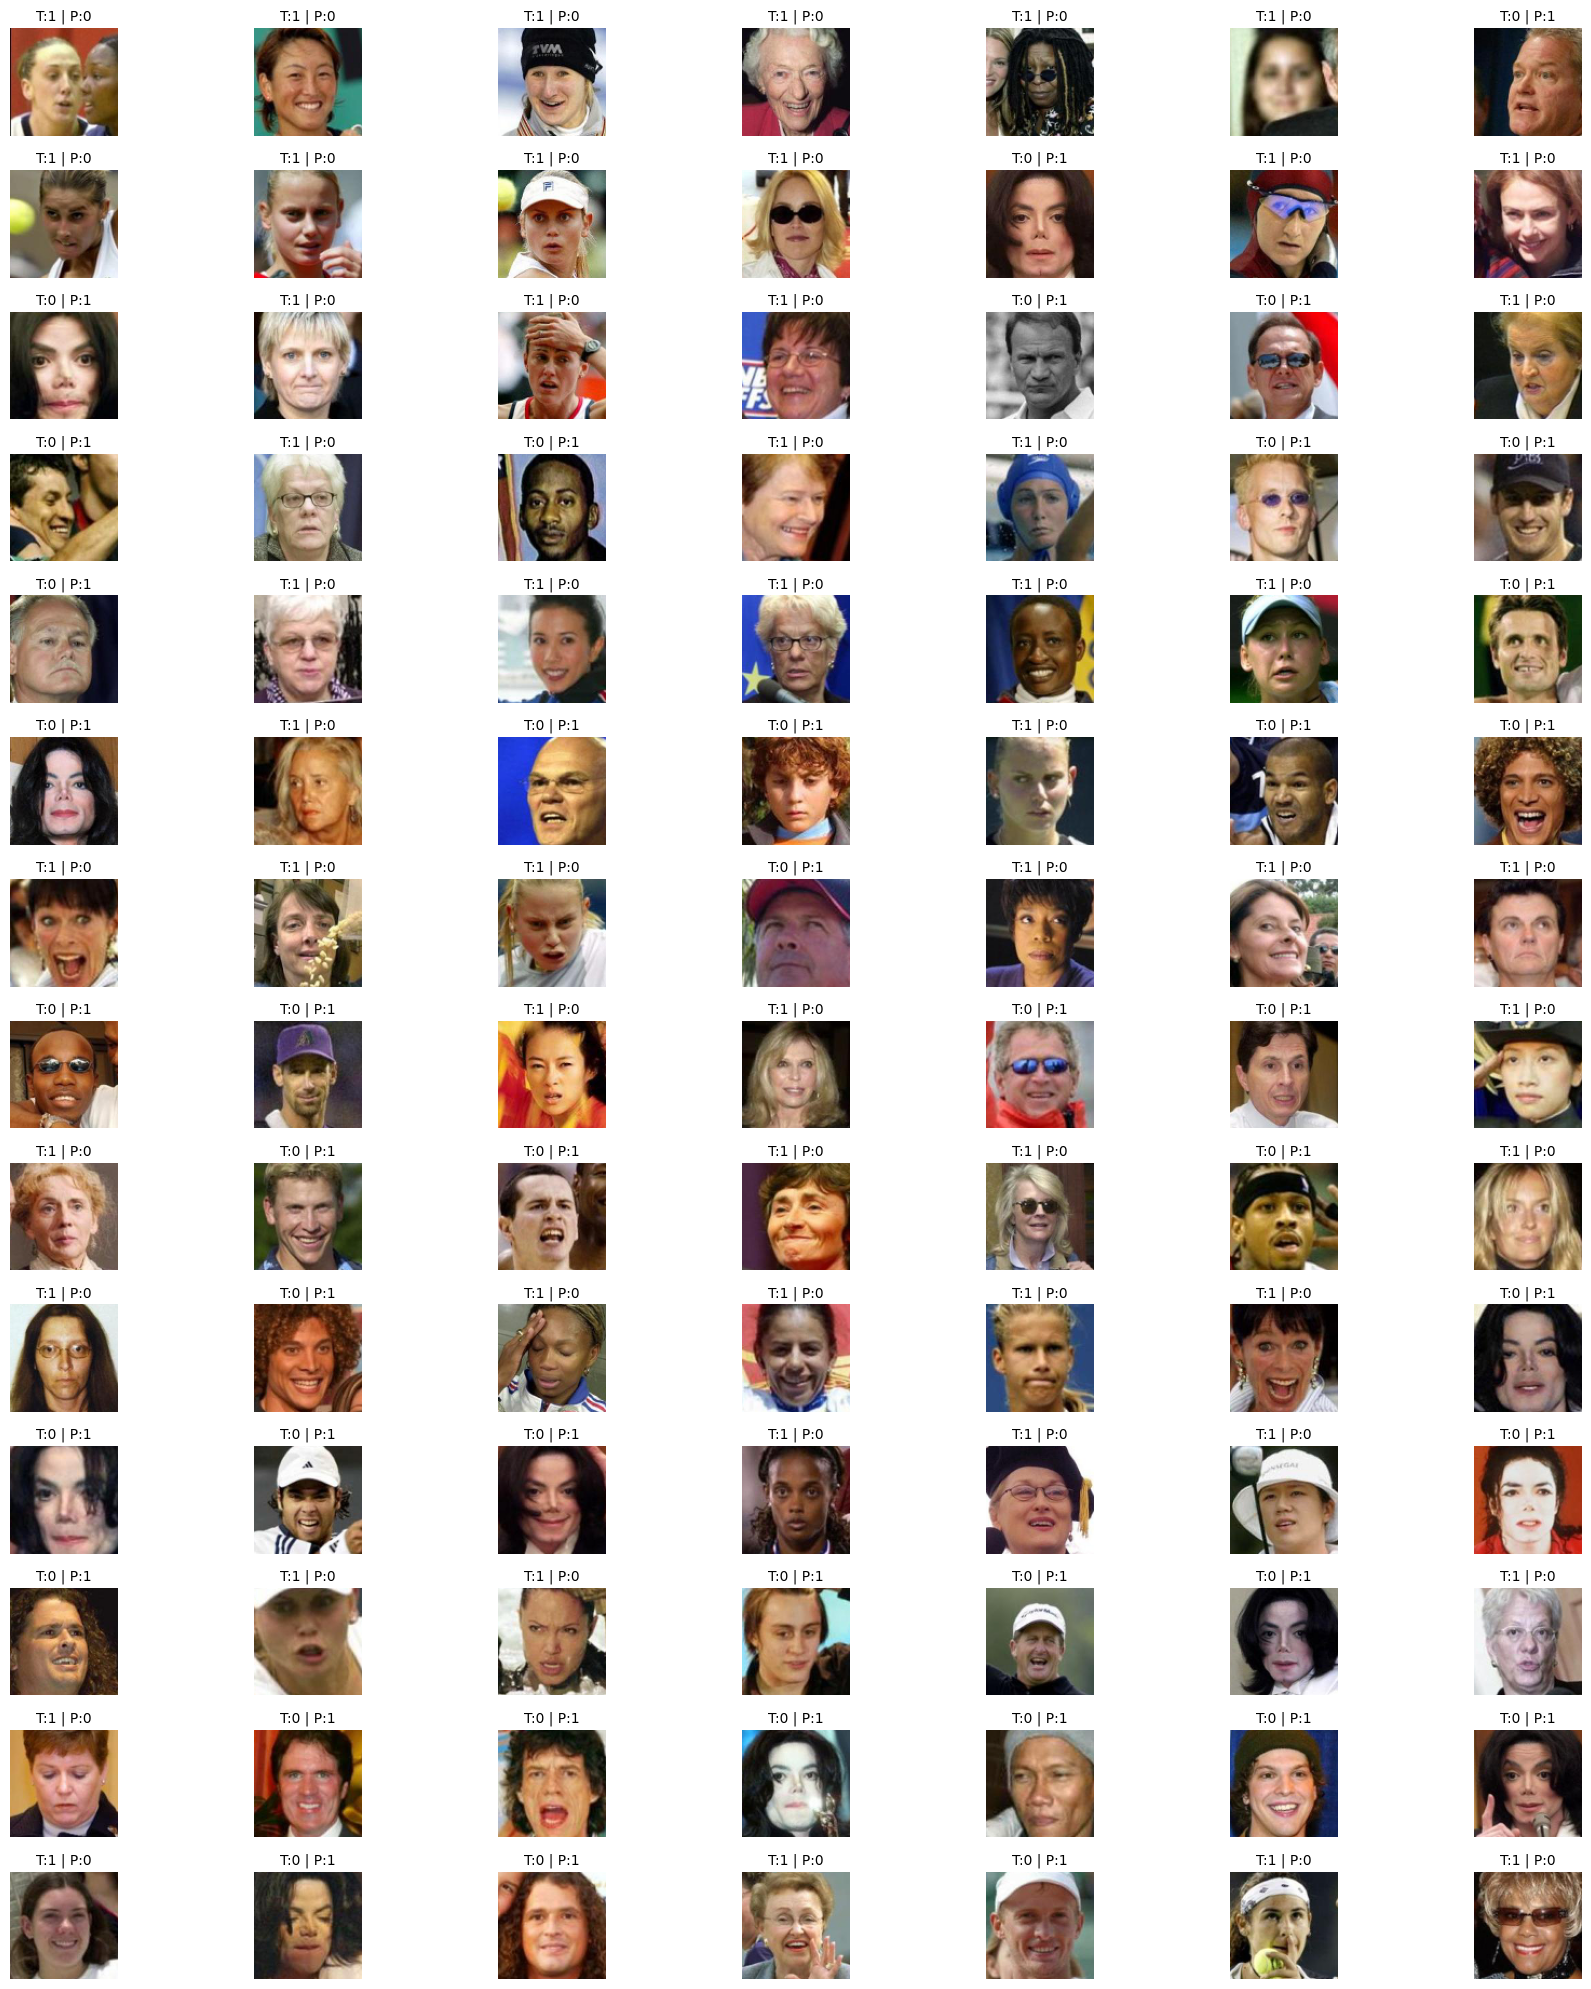
\includegraphics[width=0.85\textwidth]{images/beforebest.png} 
  \caption{Muestras fallidas por el modelo antes de aplicar ensemble}
  \label{fig:gender_samples}
\end{figure}

Si nos fijamos, a parte de no saber si Michael Jackson es hombre o mujer, el modelo también tiene problemas con personas con gafas, gorras y en general con aquellas a las que no se les ve el pelo (aun que no todos son así claro). Esto nos lleva a pensar que depende mucho de estas características para hacer la predicción, y que si no las tiene, el modelo se confunde.

Por eso, se ha implementado un \textbf{aumento de datos específico} que, a partir del concepto del RandomErasing, pretende centrarse en zonas específicas de la imagen, en concreto en la zona del pelo. Con este aumento, se consigue pasar de un 96.5\% a un 97.1\% de accuracy en validación. 

Aún así, no se ha conseguido llegar al 98\% de accuracy, por lo que ha decidido probar a ajustar el umbral de predicción y hacer inferencia usando cada imagen y su versión invertida horizontalmente. Con esto alcanzamos un 97.3\% de accuracy, solo usando este modelo.

Luego, siguiendo las indicaciones del paper, se ha implementado un ensemble de 3 modelos con diferentes seeds, AdamW, label smoothing y los data augmentation que han demostrado funcionar incluyendo la personalizada, subiendo un pelín el accuracy a 97.5\%. 

Al ver que se llegaba a un tope, se ha cambiado directamente la arquitectura del modelo. Visto que el paper llega a un tope con el setup actual, por lo que se ha usado una ResNet con 3 skip connections y dos convoluciones por bloque.

Con esta nueva arquitectura, se ha conseguido llegar a un 98.4\% de accuracy en validación, y con el ensemble de 3 modelos, se ha llegado a un 98.6\%, superando el objetivo marcado. Tras algunas pruebas se ha superado esta marca añadiendo otra capa de convolución a cada bloque, llegando a un 98.6\% con un solo modelo y a un 98.8\% con un ensemble, siendo este el mejor resultado obtenido.

\subsection{Modelo pequeño}
Para conseguir el objetivo de un modelo con menos de 100k parámetros y un accuracy de al menos 95\%, se ha optado por usar exactamente la misma arquitectura que la usada antes de la ResNet, pero esta vez usando un \texttt{AdaptiveAvgPool2d((6, 6))} como entrada a la parte densa del modelo y 61 canales en vez de 64 en la última capa convolucional, lo que a su vez reduce el número de neuronas de la primera capa densa.

Esto hace que el número de parámetros se reduzca a 99.0K, y con la misma pipeline de entrenamiento, aumento de datos y label smoothing, se ha conseguido fácilmente que el accuracy en validación se mantenga por encima del 95\%, llegando a un 96.8\%.

\begin{table}[H]
\centering
\begin{tabular}{llr}
	\toprule
	\textbf{Modelo} & \textbf{Técnica} & \textbf{Accuracy \%} \\
	\midrule
  Modelo I & Base sin \texttt{AdaptiveAvgPool2d} & 93.0 \\
	& Mejores técnicas & 96.5 \\
  & Aumento específico & 97.1 \\
  & Horizontal flipping & 97.3 \\
  & Todo + Ensemble & 97.6 \\
	\midrule
  ResNet 1 & Todo & 98.2 \\
  & Todo + Ensemble & 98.6 \\
  ResNet 2 & Todo & 98.6 \\
  & Todo + Ensemble & \textbf{98.8} \\
	\midrule
  Modelo I Pequeño & Todo & \textbf{96.8} \\
  & Todo + Ensemble* & 97.0 \\
	\bottomrule
\end{tabular}
\caption{Resultados de accuracy para diferentes técnicas aplicadas. Todo es la combinación de AdamW, label smoothing, data augmentation y aumento específico. Ensemble es la combinación de 3 modelos con diferentes seeds entrenados con esta pipeline. * Al ser 3 modelos, se supera el límite de 100k parámetros, pero cada modelo individualmente se mantiene por debajo de este límite.}
\label{tab:accuracy_ej1}
\end{table}

Como vemos, el tamaño del modelo no ha tenido tanta importancia a la hora de conseguir un buen accuracy y ha sido más la configuración del entrenamiento, los data augmentation y el buen uso del modelo en inferencia.


\section{Ejercicio 2: Car Model Identification}
Para esta tarea, partimos usando el código del ejercicio anterior, toda la pipeline de entrenamiento y data augmentation se ha mantenido (menos el aumento de datos personalizado), aunque se han ajustado algunos hiperparámetros como el learning rate.

Ahora la diferencia será que no solo usamos una CNN, sino dos y ya entrenadas. Usaremos una ResNet-50 y una VGG-16 preentrenadas en ImageNet tanto para crear una red bilineal con ambas como para solo usar una y crear redes siamesas.

\subsection{Datos}
De forma similar al ejercicio anterior, los datos venían en formato numpy y ya divididos en entrenamiento y test (validación). Se han cargado y convertido a un dataset de PyTorch para facilitar su uso en el entrenamiento de los modelos.

Ahora, estas imágenes tienen un tamaño de 250x250. Por los tamaños de las salidas de las CNNs usadas, se han reescalado a 224x224 para que su último mapa convolucional devuelva una salida de 7x7 (ambas), que es lo que se necesita para la parte bilineal del modelo.

\subsection{Entrenamiento}
Como ya sabemos, para entrenar una red bilineal usando dos CNNs ya entrenadas, únicamente tenemos que combinar las salidas de ambas CNNs, hacer un producto externo entre todos los canales de las salidas. Este tensor se proyecta a un vector y se normaliza según el tamaño del mapa convolucional, que en este caso es de 7x7, y se le aplica una raíz cuadrada seguida de una normalización L2. 

Finalmente, este vector tendrá un tamaño equivalente a multiplicar los canales de ambas redes (por ejemplo, $2048 \times 512 = 1.048.576$ características si cruzamos la ResNet y la VGG), y se pasa a una sola capa lineal que da 20 salidas, una por cada clase.

Para hacer efectivo el entrenamiento de esta red bilineal, se congelan las dos redes convolucionales, y se entrena solo la capa lineal final hasta que se estabilice. Luego, se reduce el learning rate en dos órdenes de magnitud y se descongelan las CNNs para hacer un fine-tuning de toda la red.

\subsection{Técnicas probadas}
Con el mismo proceso de entrenamiento que el ejercicio anterior, no se ha tenido que cambiar apenas nada y se han podido probar los tres posibles enfoques para esta tarea sin mucha dificultad: Una Bilinear con ResNet-50 y VGG-16, una red siamesa con ResNet-50 y otra red siamesa con VGG-16. 

\textbf{Un detalle importante:} para hacer las redes siamesas no se cargan dos modelos idénticos en memoria (lo cual sería un desperdicio enorme de recursos). Simplemente se carga la red una vez, y para sacar las características se hace el producto externo de su salida consigo misma. Luego el backpropagation se encarga de actualizar los pesos de la red para que aprenda a sacar características que sean útiles para esta tarea.


\begin{table}[H]
\centering
\begin{tabular}{lrr}
	\toprule
	\textbf{Técnica} & \textbf{Accuracy\% Fase 1} & \textbf{Accuracy\% Fase 2} \\
	\midrule
  VGG-16 siamesa & 65.94 & 68.11 \\
  ResNet-50 siamesa & 49.36 & 67.73 \\
  Bilineal VGG-16 y ResNet-50 & 65.94 & \textbf{73.72} \\
	\bottomrule
\end{tabular}
\caption{Resultados de accuracy para diferentes redes}
\label{tab:accuracy_ej2}
\end{table}

Tras el entrenamiento de solo la última capa (Fase 1), se obtenían unos resultados de accuracy bastante buenos para la VGG y la mixta, rondando el 65.94\%, mientras que la ResNet sola arrancó más floja. Luego, tras descongelar las CNNs y hacer el fine-tuning (Fase 2), la precisión subió en todos los frentes, destacando la combinación Bilineal (VGG + ResNet) que alcanzó casi un 74\%.

Como se puede observar, usar una sola CNN consigue algo menos de accuracy que juntar dos distintas. Es lógico, ya que dos arquitecturas diferentes 'ven' cosas distintas en la imagen y se complementan mejor. Sin embargo, usar una sola red juega muy a favor de reducir el uso de memoria y potencia de cálculo, lo que lo convierte en un enfoque mucho más práctico y eficiente si vamos justos de recursos.

\clearpage

\section{Ejercicio 3: Attention Visualization}

%%%%%%%%%%%%%%%%%%%%%%%%%%%%%%%%%%%%%%%%%%%%%%%%%%%%%%%%%%%%%%%%%%%%%%%%%%%%%%%
%                                                                             %
%                                BIBLIOGRAFIA                                 %
%                                                                             %
%%%%%%%%%%%%%%%%%%%%%%%%%%%%%%%%%%%%%%%%%%%%%%%%%%%%%%%%%%%%%%%%%%%%%%%%%%%%%%%
\cleardoublepage
\printbibliography

%%%%%%%%%%%%%%%%%%%%%%%%%%%%%%%%%%%%%%%%%%%%%%%%%%%%%%%%%%%%%%%%%%%%%%%%%%%%%%%
%                                                                             %
%                                 APÉNDICES                                   %
%                                                                             %
%%%%%%%%%%%%%%%%%%%%%%%%%%%%%%%%%%%%%%%%%%%%%%%%%%%%%%%%%%%%%%%%%%%%%%%%%%%%%%%

\APPENDIX


%%%%%%%%%%%%%%%%%%%%%%%%%%%%%%%%%%%%%%%%%%%%%%%%%%%%%%%%%%%%%%%%%%%%%%%%%%%%%%
%                       EJEMPLOS DE CADA TIPO DE FACTURA                     %
%%%%%%%%%%%%%%%%%%%%%%%%%%%%%%%%%%%%%%%%%%%%%%%%%%%%%%%%%%%%%%%%%%%%%%%%%%%%%%

% \chapter{Apéndice correspondencia notebooks}
% \label{appendix:notebooks}
% ...

%%%%%%%%%%%%%%%%%%%%%%%%%%%%%%%%%%%%%%%%%%%%%%%%%%%%%%%%%%%%%%%%%%%%%%%%%%%%%%%
%                              FIN DEL DOCUMENTO                              %
%%%%%%%%%%%%%%%%%%%%%%%%%%%%%%%%%%%%%%%%%%%%%%%%%%%%%%%%%%%%%%%%%%%%%%%%%%%%%%%
\end{document}

